\chapter{Git on it}

{\em\small For our purposes in MSAN, we're going to ignore most of the nontrivial capabilities that programmers use routinely, such as branching and merging. Git is extremely  complicated and would not be my first choice if it weren't for the excellent {\tt github.com}.}

\section{Introduction to revision control}

{\em Revision control} is a mechanism to track all changes to a set of files, which we typically associate with the project. The file status call a {\em repository} and at any given time, my computer has lots and lots of these repositories. 

A {\tt git} repository instance is just a directory on your disk that also happens to have a {\tt .git} (hidden) directory, which is effectively a complete database of everything that's happened to the repository since it was created with {\tt git init} (or you {\tt clone}'d it from somewhere). 

If you want to throw out the repository, just remove the entire subtree from your disk. There is no central server to notify. Every repository instance is a complete copy so you could have, for example, 10 versions of the repository cloned from an original sitting on the same disk.

After you create a repository, you can create all sorts of files in the local directories managed by git, but git ignores them until you {\tt add} them. When you add files or modify files already known to git, they are in the so-called staging area (this used to be called the index). You can have whatever other files you want laying around, such as development environment preference files. Git will simply ignore them unless you {\tt add} them. This is different than other revision control systems that insist upon knowing about and managing everything under a particular subtree. I like that feature.

\subsection{Does a solo programmer need revision control?}

If you are working solo, from a single machine, and you have a regular backup mechanism in your development environment or from the operating system like Time Machine (OS X), you can get away without a formal revision system.

There are lots of important operations that can be faked without a revision system. It's a good idea to keep track of versions of the software that work or other milestones. In the old days, people would make a copy of their project directory corresponding to important milestones like "Added feature X and it seems to work." You can do comparisons using a diff tool in between directories.

Whether your IDE does it or a revision control system does it, I find it very important to look back at recent changes to see what changes have introduced a bug. Or I decide to abandon a small piece of what's going on and flip a file back to an old version.

A good example of use of a repository is the repository for this course:

\href{https://github.com/parrt/msan501}{\textcolor{blue}{https://github.com/parrt/msan501}}

\noindent It contains all the changes that I've made since I started teaching this course.

These days, revision control systems are meant to be used among multiple computers and multiple developers, but they are still useful even on a single machine.

\subsection{Solo programmer, sharing across machines}

In order to work on that software from your home machine and a laptop for example, you have to make copies. That introduces the possibility that you will overwrite the good version of your software. Or, you will forget that you had made changes on your laptop but have now made a bunch of changes on your desktop. Resolving things can be tricky and error-prone.

As a side benefit, pushing your repository to a remote server gives you a backup automatically.

\subsection{Multiple programmers}

When you add another person to the project, people end up mailing code around but it's difficult to perform a merge. My experience watching students do this reveals that two versions of the software always appear. Both students shout that their version is better and that the other version should be abandoned.

In my experience, no matter how you try to fake multiple states of the source code and share, merging changes to work on the same code base is a nightmare.

Once in a while I go back and I look at the history of changes. Sometimes I want to know who screwed this up or I want to see the sequence of changes that I made or that were made by somebody else.

Every single commercial developer I know uses revision control at work. Every company you will encounter uses it. For that reason alone, you need to learn revision control to be functional in a commercial setting.

\section{Cloning an existing repository}

Fire up SourceTree and use the file menu {\tt New / Clone} option. You can clone that starter kit into any directory you like, but you should probably name it {\tt msan501} or something similar. Note that I'm still in the process of setting up student repositories as I'm writing this prior to receiving a list of github ids. The github URL you will clone will not be similar to {tt msan-501-starterkit} but instead {\em YourGihubUserid-msan501}.
\vspace{5mm}

\begin{marginfigure}
\begin{center}
\scalebox{1}{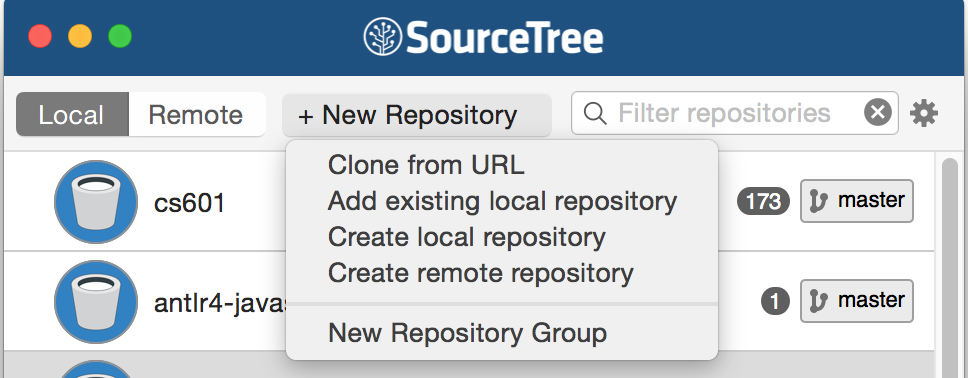
\includegraphics{figures/srctree-clone.png}}\\
\scalebox{.8}{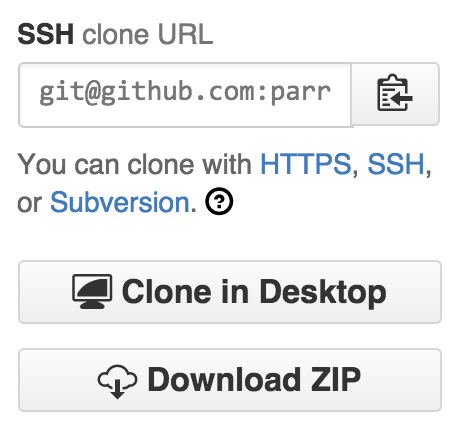
\includegraphics{figures/srctree-url.png}}\\
\scalebox{1}{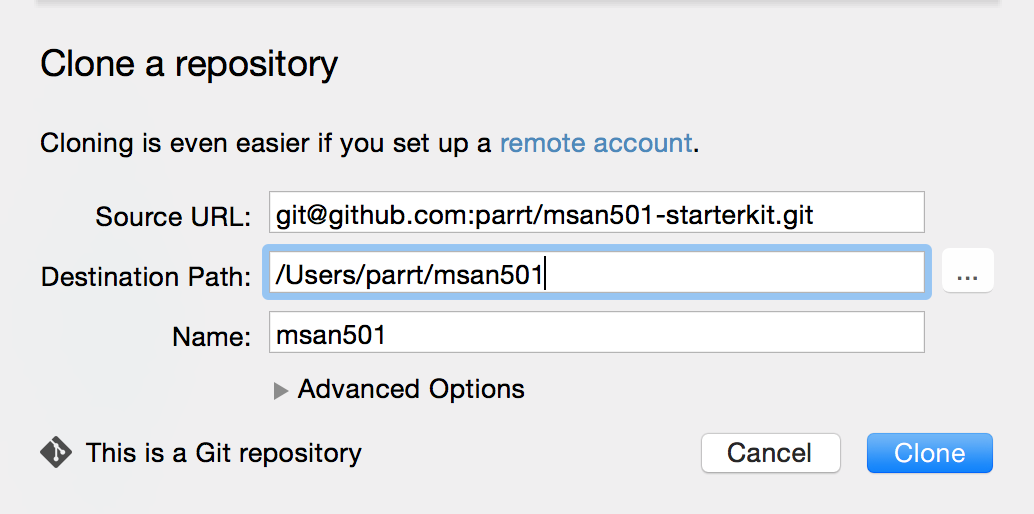
\includegraphics{figures/srctree-url2.png}}
\end{center}
\end{marginfigure}

You'll then see the status of the repository; click on the {\tt master} branch in the left gutter:
\vspace{5mm}

\scalebox{.65}{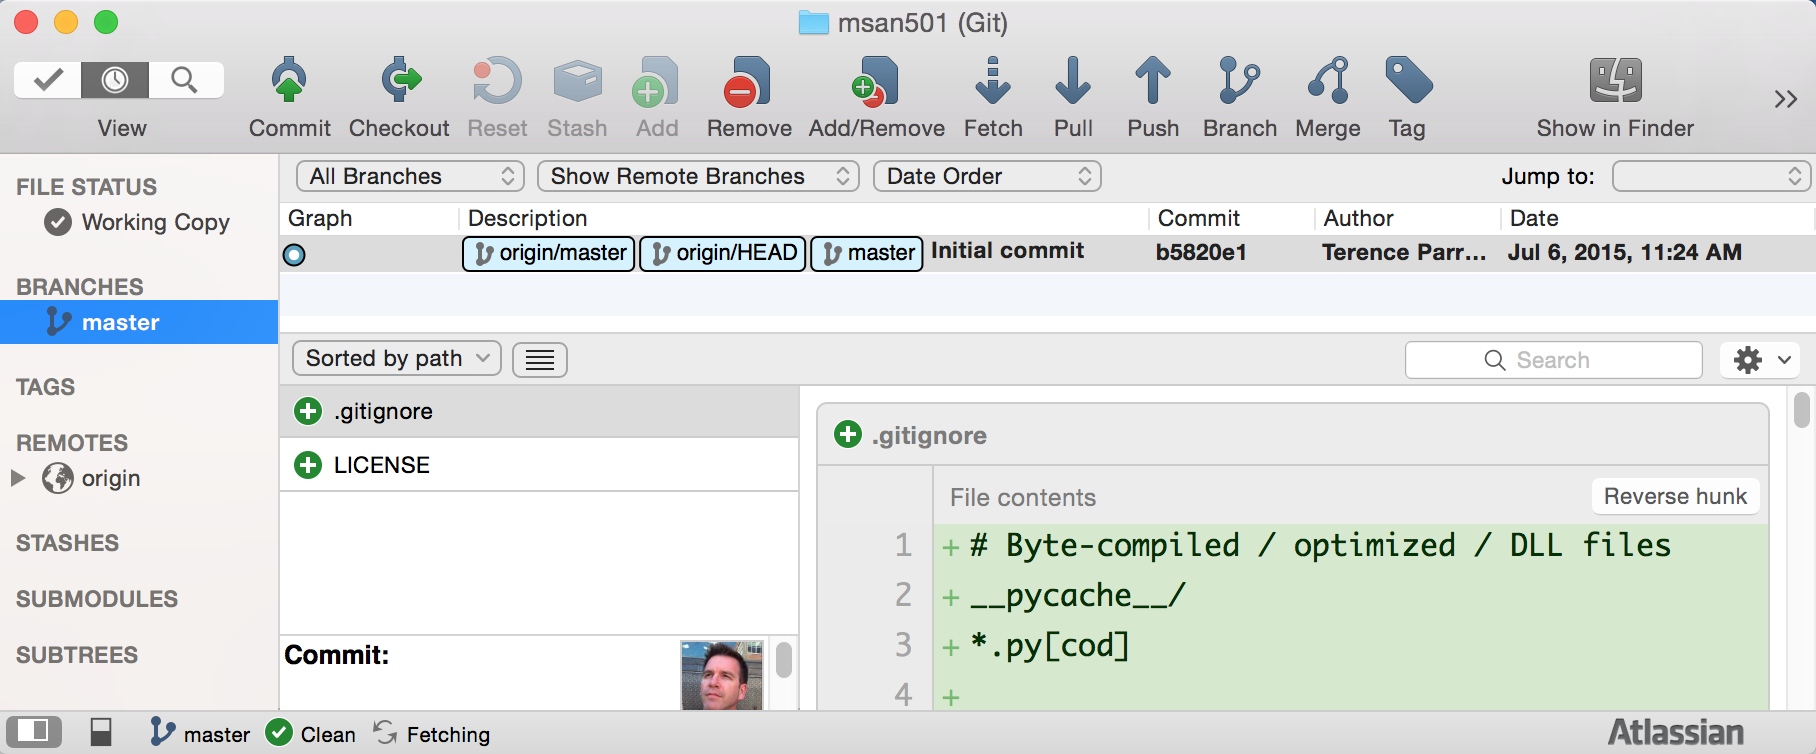
\includegraphics{figures/srctree-repo.png}}

Naturally, this is all much more explicit and quicker from the commandline:

\begin{lstlisting}[style=BashInputStyle]
$ cd ~
$ git clone git@github.com:parrt/msan501-starterkit.git msan501
\end{lstlisting}

\section{PyCharm + git = no problem}

\begin{marginfigure}[1in]
\begin{center}
\scalebox{1}{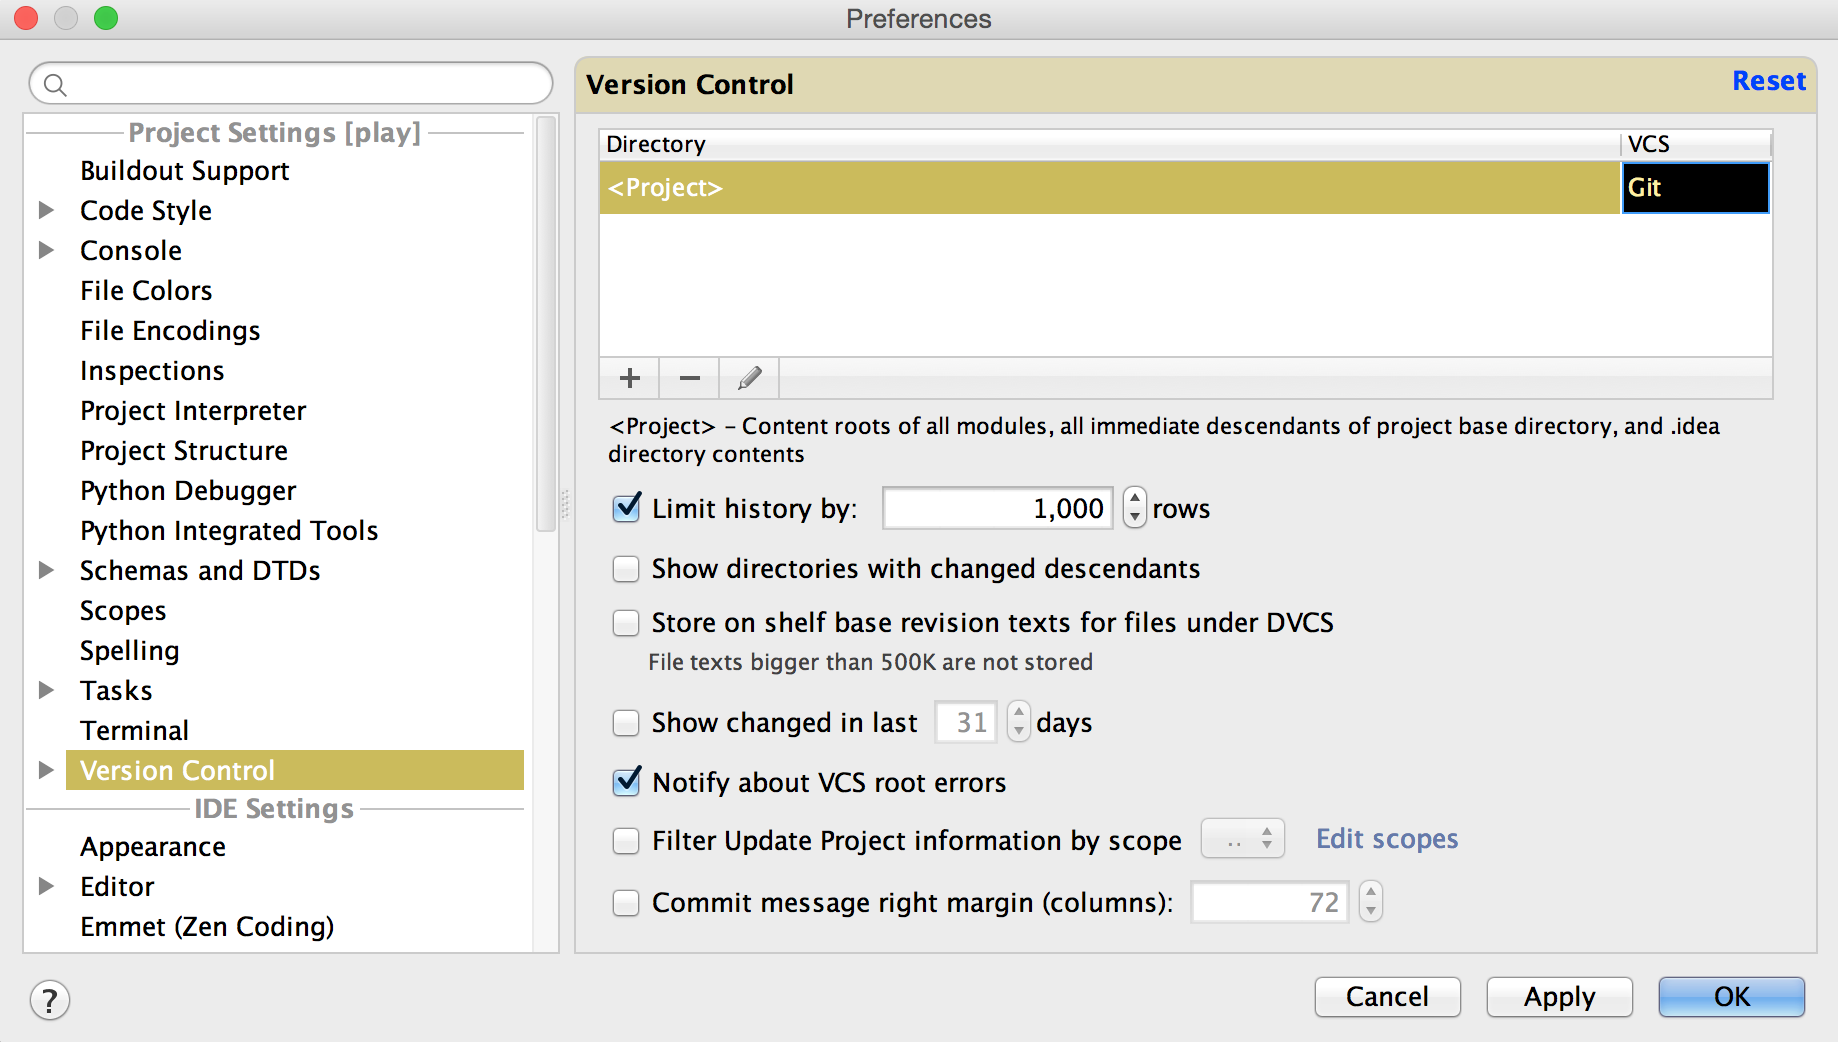
\includegraphics{figures/pycharm-git-config.png}}
\scalebox{1}{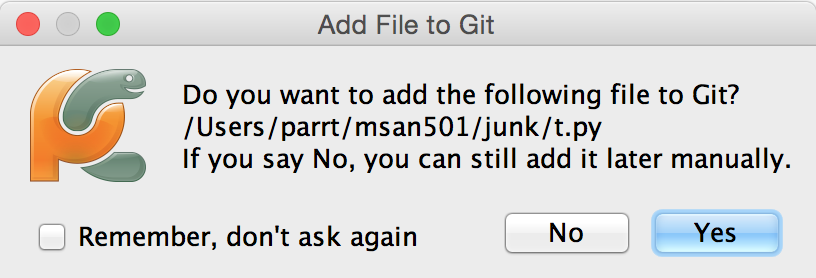
\includegraphics{figures/pycharm-git-add.png}}
\end{center}
\caption{Git config in PyCharm}
\end{marginfigure}

Most of the time, you can use PyCharm to avoid all of the unpleasantness with the specialized git commands. For example, opening PyCharm on your {\tt msan501} directory after you clone it from github should automatically detect that the directory is a repository. But, you can check this in the preferences. Then, when you create a new file, say, {\tt t.py}, PyCharm will automatically ask if you want to add it to the repository. The two snapshots in the gutter show you what it looks like. You can click the checkbox so that it always just adds files. If you want to manually add them later it's okay. You can do so under the VCS (version control system) menu.

To figure out what changes you have made to the existing repository, click on the Changes tab at the bottom of PyCharm. You will see that t.py is a change (addition) to the repository.

\begin{marginfigure}
\begin{center}
\scalebox{1}{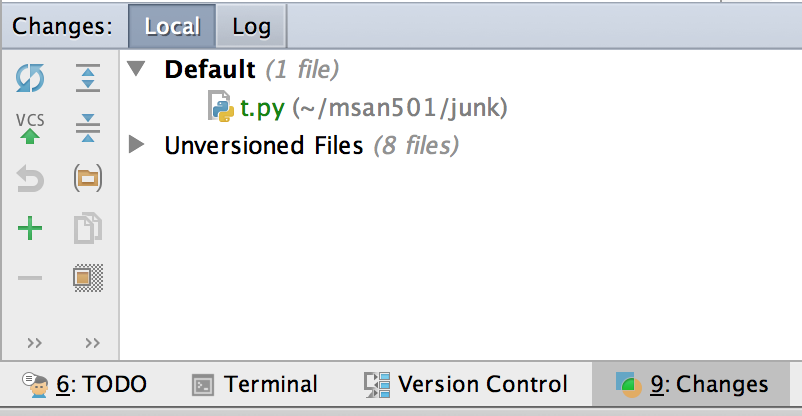
\includegraphics{figures/pycharm-git-changes.png}}
\end{center}
\caption{View changes to repo}
\end{marginfigure}

Use menu option VCS > Commit Changes to commit your changes to the local repository.   As part of the commit, you can push to the {\tt origin}, which will bring up the Git Push dialog box.
\vspace{5mm}

{\bf Tagging}.  As part of delivering your projects, you will signal to me that a particular task is ready for review by tagging. The specific tag name will identify which project I should review and then I will add a tag to indicate I have graded it.  Going back to SourceTree, we can see the recent commit of t.py. Right clicking on that line in the GUI, brings up a menu where we can add a tag. The tag will be added to the local repository and pushed to the origin if you click the appropriate checkbox. I will not be able to see it until he goes back to the origin.

\begin{marginfigure}
\vspace{-1in}
\begin{center}
\scalebox{1}{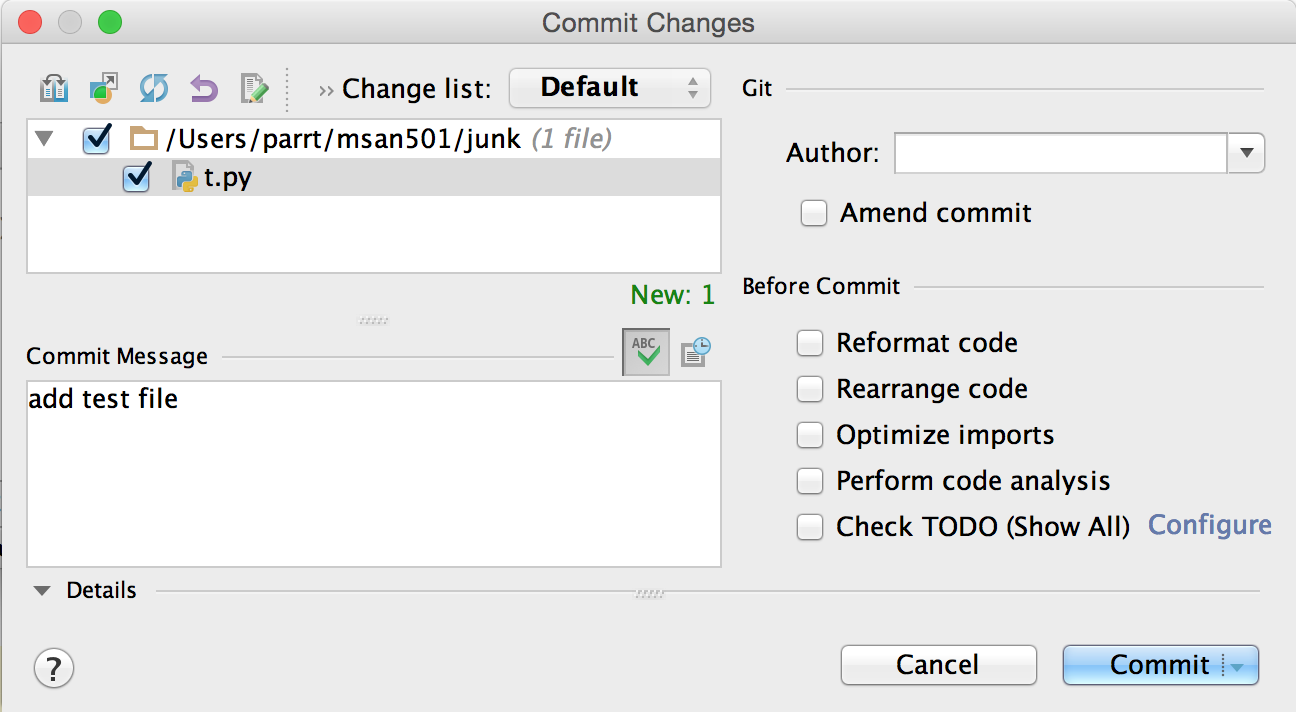
\includegraphics{figures/pycharm-git-commit.png}}
\scalebox{.8}{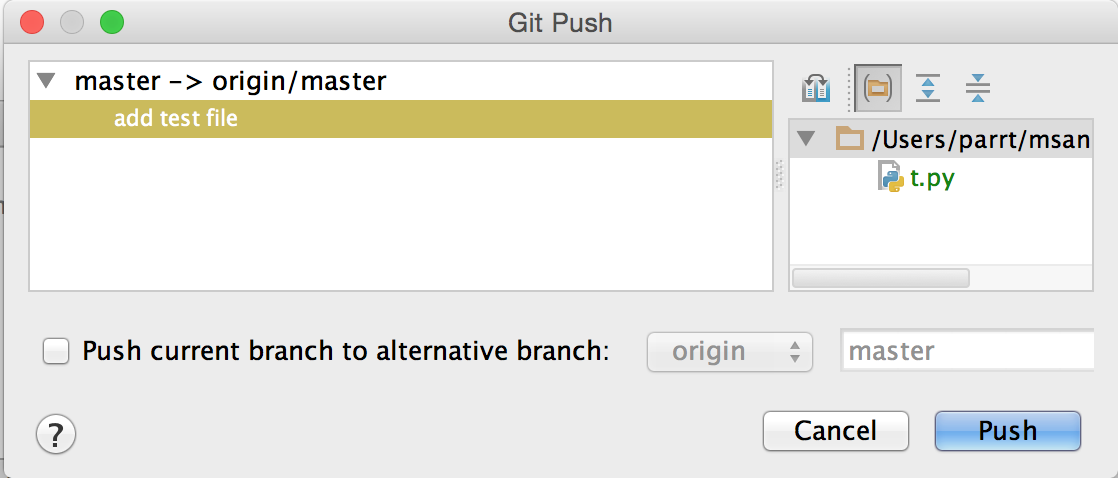
\includegraphics{figures/pycharm-git-push.png}}
\end{center}
\caption{Commit and push}
\end{marginfigure}

\begin{marginfigure}
\begin{center}
\scalebox{1}{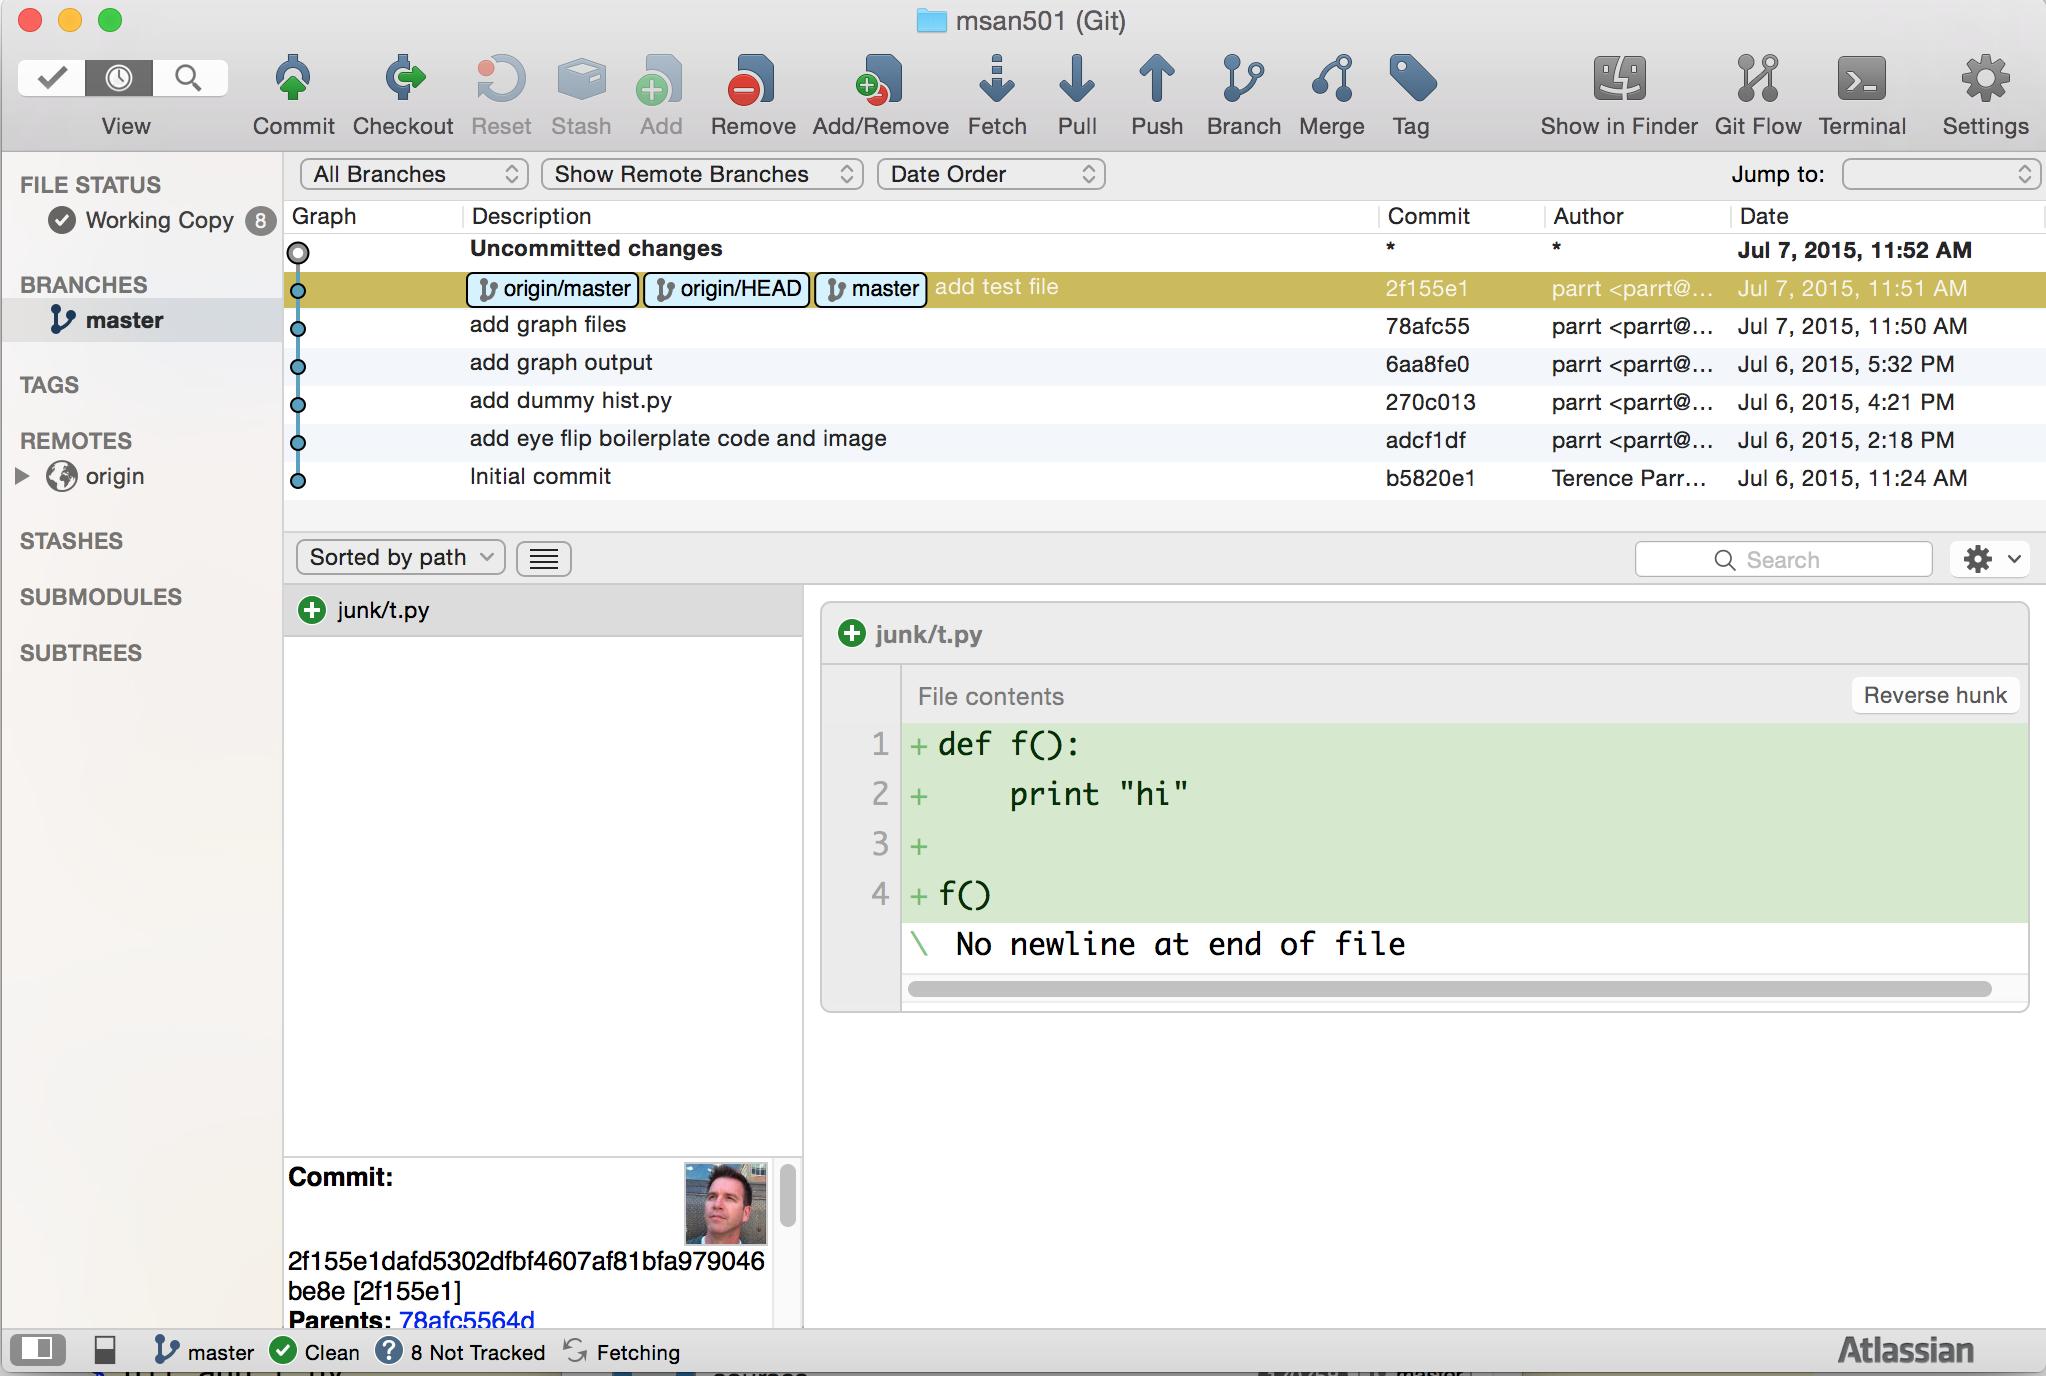
\includegraphics{figures/srctree-pycharm-add.png}}
\scalebox{.8}{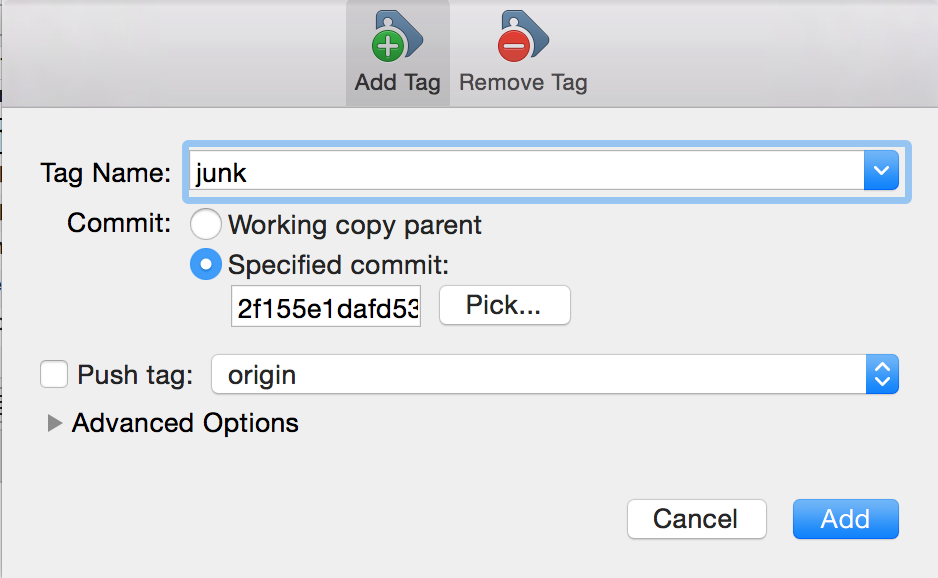
\includegraphics{figures/srctree-tag.png}}
\end{center}
\caption{SourceTree view, tagging}
\end{marginfigure}

\section{Git from the command line}

{\bf Adding to repo}. To add files, just create them and do a {\tt commit}:

\begin{lstlisting}[style=BashInputStyle]
$ cd ~/msan501
$ mkdir junk
$ cd junk
... create t.py ...
$ git add t.py
$ git commit -a -m 'initial add'
\end{lstlisting}

\noindent {\bf Make changes}. Then you can make changes and do another commit. Make sure use the {\tt -a} command. By the way, deleting a file is also considered a change but you can also use {\tt git rm} {\em filename}.

\noindent {\bf Checking differences with repo}. If you make a change and want to know how it's different from the current repository version, just use diff:

\begin{lstlisting}[style=BashInputStyle]
$ ... tweak t.py ...
$ git diff t.py
...
\end{lstlisting}

\noindent {\bf Reverting}. If you screw up and want to toss out everything from the last commit, do a reset and make sure you use the hard option:

\begin{lstlisting}[style=BashInputStyle]
$ ... tweak whatever you want ...
$ git reset --hard HEAD
\end{lstlisting}

\noindent which throws out all changes since the last commit. If all you want to do is revert uncommitted changes to a single file, you can run this:

\begin{lstlisting}[style=BashInputStyle]
$ git checkout -- filename
\end{lstlisting}

I think they call that funny dash-dash option ``sparse mode.'' See? Git is the assembly code of revision systems. blech.

\noindent {\bf Correcting commit message}. One of the other things I often have to do is to fix the commit message that I just wrote in a commit command.

\begin{lstlisting}[style=BashInputStyle]
$ git commit --amend -m "I really wanted to say this instead"
\end{lstlisting}

\noindent {\bf Adding file you forgot to commit}. If you forgot to add one of the files and you wanted in a previous commit, you can also use amend. Just add the file and use amend:

\begin{lstlisting}[style=BashInputStyle]
$ git add t2.py
$ git commit --amend --no-edit
\end{lstlisting}

{\bf Checking working dir and staging area vs repo.} Finally, if you want to figure out what changes you have made such as adding, deleting, or editing files, you can run:

\begin{lstlisting}[style=BashInputStyle]
$ git status
On branch master
Your branch is up-to-date with 'origin/master'.

Untracked files:
  (use "git add <file>..." to include in what will be committed)

    t3.py

nothing added to commit but untracked files present (use "git add" to track)
\end{lstlisting}

\section{Don't fear {\tt commit}ment}

Every time you {\em commit} a change (file edit, file add, file delete, ...) to the repository, the revision control system tracks a patch called the {\em diff} that indicates essentially how to edit the first file version in order to arrive at the current file version. Storing just the differences is very space efficient and  lets the revision control system apply the same set of changes to a file on a different computer to keep them both in sync.  

Having a complete list of changes is extremely useful. For example, here is a chunk taken out of the middle of my commits on the ANTLR repository as shown by SourceTree:

\scalebox{.85}{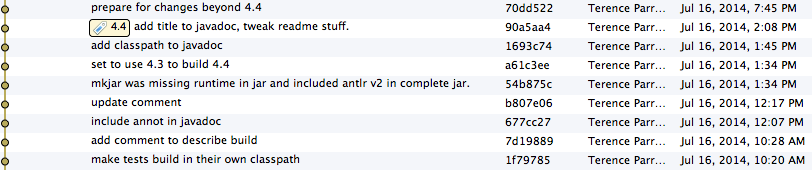
\includegraphics{figures/commits.png}} 

That should look very much like Time Machine on OS X to you. You can go back and look at changes made to the repository for any commit.

You will also notice that I have tagged a particular commit as 4.4 with the tag command. This makes it easy for me to flip the repository back to a specific commit with a name rather than one of those funky commit checksums.

You should commit only logical chunks like feature additions, bug fixes, or comment updates across the project, etc.

Commit messages are important. Do not use meaningless messages, as I see students sometimes do:

\begin{alltt}
Add t.py
Alter t.py
Change t.py
...
\end{alltt}

I have even seen git commit messages: {\tt one}, {\tt two}, {\tt three}. Nothing spells laziness or academic dishonesty than that.

In rare cases, when I'm working alone, I sometimes use a private repository as a means of sharing files across multiple computers like dropbox. In this case, my commits are just to take a snapshot to pull it down on another machine. The commit message doesn't matter (though I might still look back through the changes at some point). When doing this for a real project, it's best to use stash per the next section.

\section{With a remote server like github}

When you're working by yourself (and without branches), a remote server acts like a central server that you can push and pull from. For example, I push from my work machine and pull to my home machine or my laptop. And then reverse the process with changes I make at home over the weekend.

For example, once I have commit all of my changes that work and I'm ready to go home, I push to the origin:

\begin{lstlisting}[style=BashInputStyle]
$ git push origin master
\end{lstlisting}

\noindent From home, I do:

\begin{lstlisting}[style=BashInputStyle]
$ git pull origin master
\end{lstlisting}

\noindent The origin is the alias for the original server we cloned from and master is our master branch, which we can ignore until we look at branches.

To look at the remote system alias(es), we use:

\begin{lstlisting}[style=BashInputStyle]
$ git remote -v
origin  git@github.com:parrt/msan501.git (fetch)
origin  git@github.com:parrt/msan501.git (push)
\end{lstlisting}

